\section{Depth and ego motion prediction}

This section explains the implementation that was done in this thesis project for the depth and ego motion predicting networks.

\subsection{Architectures for depth and ego motion CNNs}

In order to predict depth and motion from monocular images two different CNN architectures are examined. Both are encoder-decoder type architectures, and their general layout is illustrated in Figure \ref{fig:net}.

The first architecture is referred to as SfMlearner\cite{sfmlearner}. It uses a DispNet\cite{dispnet} architecture to predict depth maps at four different scales.

The second architecture is referred to as Monodepth2\cite{monodepth2}. It uses a ResNet18 architecture instead of a DispNet architecture to predict depth estimates. This architecture is smaller resulting in faster training and evaluation.

Both SfMlearner and Monodepth2 uses a separate network to predict poses between frames. The pose network has a ResNet18\cite{resnet} architecture, but the decoder is modified to predict pose updates in an Euler-angle-axis representation.

\begin{figure}[H]
	\centering
	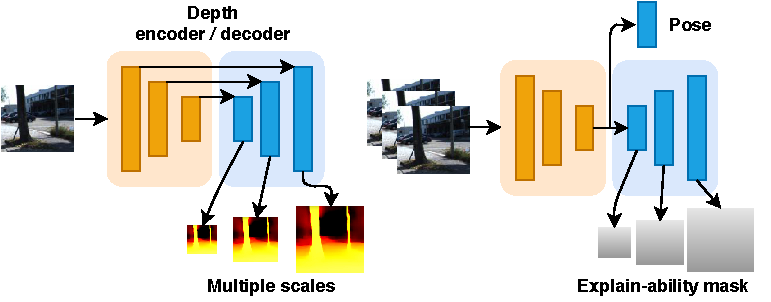
\includegraphics[width=1.0\textwidth]{net}
	\caption{High level diagram of the network architectures used for depth and ego motion prediction. The layers from the depth encoder are concatenated into the layers of the decoder. Depth maps are computed at multiple scales in the decoder and are all used in the loss function. A separate network that takes as input 3 subsequent frames predicts the poses $\textbf{T}_{t\rightarrow t-1}$ and $\textbf{T}_{t\rightarrow t+1}$ between the target and nearby reference frames. The pose network shares encoder with the explain-ability mask predicting network (section \ref{sec:modellimit}).}
	\label{fig:net}
\end{figure}

\subsection{Differentiable depth image warping}
\label{sec:diffwarp}

The core component of unsupervised depth learning is the differentiable depth image warp operation in the loss function of the CNN networks. The goal is to reconstruct the target image from pixel values in the source image using the predicted depth and ego motion. If the predictions are good, then the reconstruction will also be good. If the loss is based on the quality of the reconstruction then the loss will be a good measure on how well the network has learned to predict depth and ego motion. To perform the reconstruction we need a few components. Firstly the intrinsic camera matrix:

\begin{equation}
\textbf{K} = 
\begin{pmatrix}
f_\mathrm{x} & s & x_0 \\
0 & f_\mathrm{y} & y_0 \\
0 & 0   & 1
\end{pmatrix}
\end{equation}

where $f$ is the focal length, $s$ is the skew coefficient (often zero), and $x_0$ and $y_0$ represent the principal point. Secondly we need the the predicted depth $ \textbf{D}_t(\textbf{p}_t) $ of pixel $ \textbf{p}_t $ of the target (current) frame. Thirdly we need the predicted ego motion in the form of a transform matrix $ \textbf{T}_{t \rightarrow s} $ from the target to the source (next or previous) frame in the sequence:

\begin{equation}
\textbf{T}_{t \rightarrow s} =
\begin{pmatrix}
\textbf{R} & \textbf{t} \\
0 & 1
\end{pmatrix}
\end{equation}

Given these, we can project the position of the target pixel $ \textbf{p}_t $ onto the source image $\textbf{I}_s$. We call this new position $ \textbf{p}_s $, and it is calculated in homogeneous coordinates as:

\begin{equation}
\textbf{p}_s \sim 
\begin{pmatrix}
\textbf{K}  & \textbf{0} \\
\end{pmatrix}
\textbf{T}_{t \rightarrow s} \textbf{D}_t(\textbf{p}_t) \textbf{K}^{-1} \textbf{p}_t 
\end{equation}

The pixel position $ \textbf{p}_s $ is however continuous and in order to sample the discrete source image $ \textbf{I}_s $ a differentiable bilinear sampling method is used\cite{spatialtransformernetworks}. The value at the continuous sampling point $\textbf{p}_s$ is interpolated from its four discrete neighbors. This process is illustrated in Figure \ref{fig:warp}.


\begin{figure}[H]
	\centering
	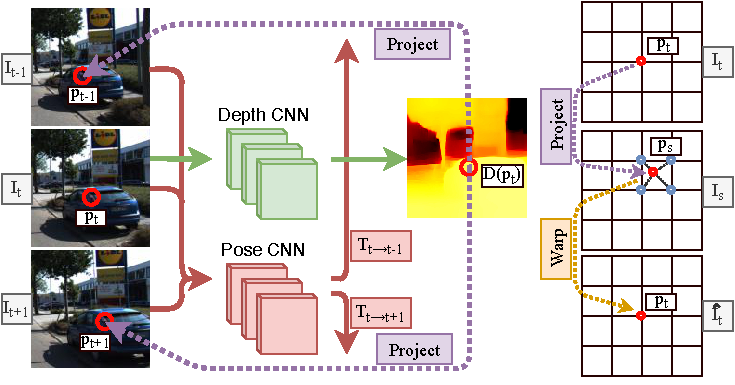
\includegraphics[width=1.0\textwidth]{warp}
	\caption{The \abbrCNN predicts the depth map $\textbf{D}$ of the target image $\textbf{I}_t$, and also the relative movement, $\textbf{T}_{t\rightarrow t-1}, \textbf{T}_{t\rightarrow t+1}$ between the target image and the source images. Each pixel $p_t$ in the target image is projected onto a position in the source images which are sampled using bilinear interpolation. This should recreate the appearance of the target image but with pixels sampled from the source image. An appearance similarity metric between the original target image and the recreated target images can be used as the loss function for the \abbrCNN to learn to accurately predict correct depth and movement.}
	\label{fig:warp}
\end{figure}

%TODO: Insert examples of warped/recreated and diff images between target and recreated images.....


\subsection{Loss functions}
\label{sec:loss}

In order to learn the objective of depth and ego motion prediction, different combinations of the following loss terms where evaluated.

To measure the similarity of the target image $\textbf{I}_t$ and the reconstructed image $\hat{\textbf{I}}_t$ a photometric loss term defined as the mean of the absolute value of the difference of pixel intensities of the two images was used.

\begin{equation}
\mathcal{L}_p(\textbf{I}_t, \hat{\textbf{I}}_t)=\mean(|\textbf{I}_t - \hat{\textbf{I}}_t|)
\end{equation}

Another photometric loss term evaluated in this thesis is based on structured similarity, referred to as SSIM\cite{ssim}. It was originally developed to measure the quality of digital television, comparing a compressed digital image to the original distortion-free image.

\begin{equation}
\mathcal{L}_{ssim}(\textbf{I}_t, \hat{\textbf{I}}_t)=\mean(\clamp(\textbf{0},\textbf{1},\dfrac{\textbf{1}-\SSIM(\textbf{I}_t, \hat{\textbf{I}}_t)}{2}))
\end{equation}
\begin{equation}
\SSIM(\textbf{X},\textbf{Y})=\frac{(2\mu_{\textbf{X}}\mu_{\textbf{Y}}+C_1)(2\sigma_{\textbf{XY}}+C_2)}{(\mu_{\textbf{X}}^2+\mu_{\textbf{Y}}^2+C_1)(\sigma_{\textbf{X}}^2+\sigma_{\textbf{Y}}^2+C_2)}
\end{equation}

with $C_1=1e-4$ and $C_2=9e-4$. To compute the per-patch mean $\mu_{\textbf{X}}$ and standard deviation $\sigma_{\textbf{X}}$, a 1 pixel reflection padding was first used on the edges of the input images and then a $3\times3$ average pool filter with stride 1 was used to get the mean. Then $ \sigma_{\textbf{X}}=\mu_{\textbf{X}^2}-\mu_{\textbf{X}}^2 $.

The two above mentioned photometric loss terms can also be combined and balanced using $ \mathcal{L}_{ps}(\textbf{I}_t, \hat{\textbf{I}}_s) = \alpha \mathcal{L}_{ssim} + (1-\alpha) \mathcal{L}_p $. In the experiments of this thesis $\alpha=0.85$ was used, which is the same value used in the original Monodepth2 paper. As the network learns over time to predict more accurate depth and ego motion, the reconstruction loss will decrease. The loss per individual pixel is illustrated in Figure \ref{fig:diff}, which shows the loss from the same sample but after 1 and 30 epochs of training respectively.

\begin{figure}[H]
	\centering
	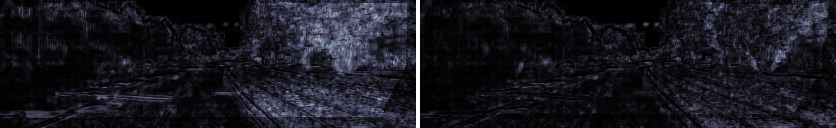
\includegraphics[width=1.0\textwidth]{diff}
	\caption{The images illustrates the photometric reconstruction loss $ \mathcal{L}_{ps} $ for each pixel in a reconstructed image for the same frame but after different length of training. The left image shows the loss after 1 epoch of training and the right image shows the loss after 30 epochs. The reconstruction loss should decrease during training as the network learns to predict better depth maps, which is what we see.}
	\label{fig:diff}
\end{figure}

To propagate the depth from textured regions to regions of uniform color a depth smoothness loss term is used. The first alternative is a loss on the second derivative of the depth intensities. This loss term will discourage the network to predict fluctuating depth values in regions of uniform color such as the pavement, that should be smooth. The drawback of this technique is that changes in depth values are penalized equally in regions where there are a lot of detail that therefore could be lost in the depth map.

\begin{equation}
\mathcal{L}_{smooth}(\textbf{D}_t)=\mean(|\delta_x^2 \textbf{D}_t|+|\delta_y^2 \textbf{D}_t|)
\end{equation}

The second alternative investigated was an edge aware smoothness loss that weights the first order derivative of the depth map with the exponential of the first derivative of the pixel intensities. This method allows large changes in depth near sharp features in the image but penelizes changes in depth in smooth regions, see Figure \ref{fig:edge}. The method showed great promise, resulting in sharper edges because the smoothness term is weighted to mostly affect areas with small intensity derivative.

\begin{equation}
\mathcal{L}_{edge}(\textbf{D}_t)=\mean(|\delta_x \textbf{D}_t|e^{-|\delta_x \textbf{I}_t|} + |\delta_y \textbf{D}_t|e^{-|\delta_y \textbf{I}_t|})
\end{equation}

\begin{figure}[H]
	\centering
	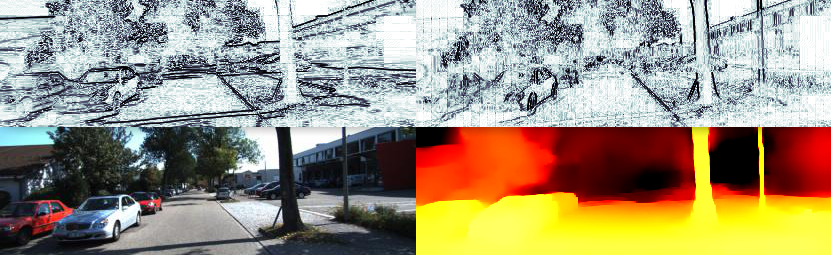
\includegraphics[width=0.9\textwidth]{edge}
	\caption{The top row of images illustrates the edge weighting terms $e^{-|\delta_y \textbf{I}_t|}$ and $e^{-|\delta_x \textbf{I}_t|}$ respectively. The weight is near 0 at the edges of tree trunks and near 1 on the pavement. This will preserve the details in the depth map around trees but keep the pavement smooth.}
	\label{fig:edge}
\end{figure}

\subsection{Depth map normalization}\label{sec:normalization}

The predicted depth is scale invariant which can make it difficult to balance the loss terms with the correct weights. To alleviate this is issue the depth map can be normalized before it is used in the loss.

\begin{equation}
\hat{\textbf{D}_t} = \frac{\textbf{D}_t}{\median(\textbf{D}_t)} 
\end{equation}

\subsection{Depth map up-scaling}\label{sec:upscale}

The smaller depth maps in the depth decoder of the network are all used in the loss. Early work in this area down-scaled the target image to fit the size of the smaller depth maps when used in the loss function. But in MonoDepth2\cite{monodepth2} it was proposed to instead up-scale the depth maps to the original target image size, see Figure \ref{fig:upscale}.

\begin{figure}[H]
	\centering
	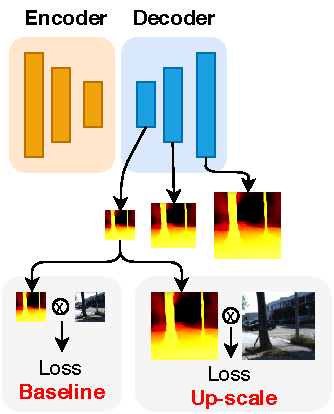
\includegraphics[width=0.3\textwidth]{upscale}
	\caption{The depth maps can optionally be up-scaled in the loss function.}
	\label{fig:upscale}
\end{figure}

\subsection{Handling occlusions}
\label{sec:occlusion}

\iffalse
\paragraph{Disparity loss} To encourage background depths (low disparities) in shadows of the depth map where occlusion has occurred a penalty on the disparity can be added $ \mathcal{L}_{o} =|d_t|. $
\fi

In the SfMLearner paper the photometric loss is calculated for the previous and next frames compared to the current in the sequence. The pixel-wise average across the frames is then used. This causes problems if a pixel is for example occluded in the previous frame, but visible in the current and next frame. In this situation the average loss will be large even though a correct depth and transformation has been predicted, because of the occluded pixel. Instead Monodepth2 suggests to pick the minimum per pixel error over the frames which alleviates this issue, see Figure \ref{fig:min}. Both techniques where implemented in this thesis and compared in the experiments.

\begin{figure}[H]
	\centering
	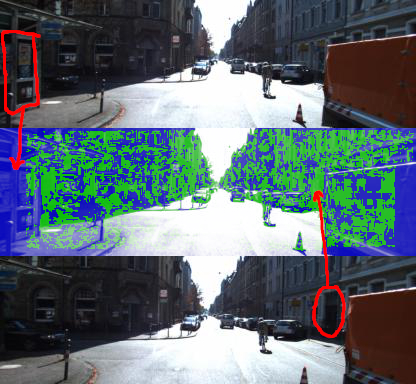
\includegraphics[width=0.5\textwidth]{min}
	\caption{By picking the per pixel minimum reprojection error the issue created by occluded pixels can be alleviated. The top image is the previous frame, the middle image is the current target frame and the bottom image is the next frame in the sequence. If the minimum reprojection error can be found in the previous frame then it is colored blue, if its from the next frame it is green. Because the door to the right is occluded by the orange truck in the previous frame, the reprojection loss from the next frame is used instead where the door is visible. The wall to the left is outside the boundaries of the next image, so the reprojection error from the previous frame is used instead.}
	\label{fig:min}
\end{figure}

\subsection{Handling model limitations}
\label{sec:modellimit}

In order to optimize using the photometric reprojecton error as the loss function two assumptions must hold. Firstly the scene must be static, meaning all objects in the scene must be still except the moving camera. Dynamic objects will cause problems. Secondly there must be photometric consistency between frames for the photometric error to make sense. This means that non Lambertian surfaces, change in lighting, and change in exposure between frames will cause problems. Two different methods of dealing with this issue was implemented and evaluated in this thesis.

\paragraph{Explainability mask} The authors of \cite{sfmlearner} tackle the model limitations by having a CNN predict what pixels are valid to use in the photometric loss function, see Figure~\ref{fig:exp}. It shares the encoder of the pose predicting network but branches of into a different decoders which estimates a mask of the valid/explainable pixels. The loss function for the mask is the cross entropy loss compared to a mask filled with ones. The photometric loss function is augmented to include the explainability mask removing pixels that cannot be explained by the predicted depth and transformation. This encourages the mask to be filled with ones, but allows some slack due to pixels that can not be explained by the photometric loss.

\begin{figure}[H]
	\centering
	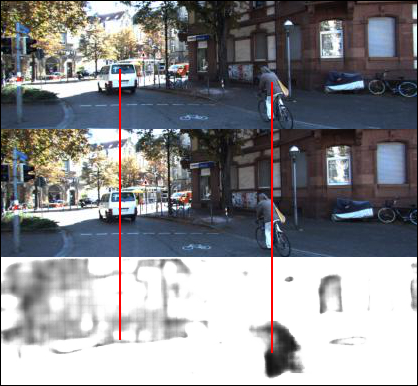
\includegraphics[width=0.5\textwidth]{exp}
	\caption{This is an image extracted from the experiments in this thesis. The top image is frame $\textbf{I}_t$ the middle image is frame $\textbf{I}_{t-1}$ and the last image is the explain-ability mask. It is visible that the network correctly predicts that the bicycle is not moving in relation to the camera, but it does not remove pixels from the white van as it should.}
	\label{fig:exp}
\end{figure}

\paragraph{Stationary pixels mask} The authors of \cite{monodepth2} introduced a mask to remove stationary pixels from the set of previous, current and next frame. This is done by creating a mask where the photometric error is smaller before applying the projection than after. This works because pixels from objects that have not moved in relation to the camera will of course have a small photometric loss without reprojection. This will remove pixels from the car dashboard and also nearby vehicles that are traveling at the same speed, see Figure \ref{fig:stat}.

\begin{figure}[H]
	\centering
	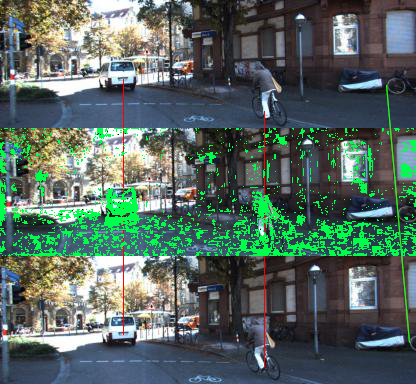
\includegraphics[width=0.5\textwidth]{stat}
	\caption{The black pixels in the image are the ones removed because their photometric error is smaller before warping the image using the depth map compared to after warping. The red horizontal lines on the van and bicyclist illustrates that they do not move with respect to the camera, and the green slanted line illustrates that the bike leaning on the wall is moving with respect to the camera. The mask successfully removes pixels on the van and bicyclist, but also removes some pixels on the pavement that should not be removed.}
	\label{fig:stat}
\end{figure}